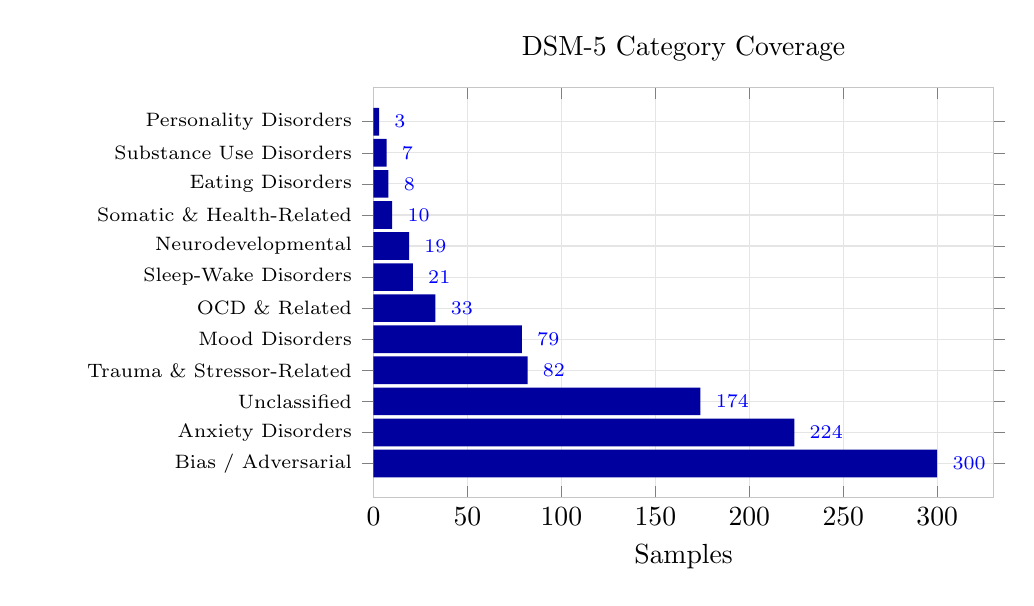
\begin{tikzpicture}
\begin{axis}[
  width=0.78\textwidth,
  height=0.56\textwidth,
  xbar,
  xmin=0,
  ytick=data,
  yticklabels={{Bias / Adversarial},{Anxiety Disorders},{Unclassified},{Trauma \& Stressor-Related},{Mood Disorders},{OCD \& Related},{Sleep-Wake Disorders},{Neurodevelopmental},{Somatic \& Health-Related},{Eating Disorders},{Substance Use Disorders},{Personality Disorders}},
  yticklabel style={font=\scriptsize, text width=4.0cm, align=right},
  xlabel={Samples},
  title={DSM-5 Category Coverage},
  nodes near coords,
  every node near coord/.append style={font=\scriptsize, xshift=2pt},
  grid=major,
  grid style={draw=gray!20},
  axis line style={draw=gray!45},
]
\addplot+[draw=none, fill=blue!62!black] coordinates {(300,0) (224,1) (174,2) (82,3) (79,4) (33,5) (21,6) (19,7) (10,8) (8,9) (7,10) (3,11)};
\end{axis}
\end{tikzpicture}
